\section{Modalità di esecuzione dei test}
In questa sezione si andrà ad analizzare le performance delle tre soluzioni VPN descritte nei capitoli precedenti, al fine di valutare quale di esse offre le prestazioni migliori.
Le prestazioni verranno valutate analizzando il throughput, la sua stabilità e la percentuale di packetloss.
I software che sono stati utilizzati per effettuare le misurazioni questi dati sono \texttt{iperf3} e \texttt{mrt}.

\subsection{Panoramica di \texttt{iperf3}}
Ancora del testo

\subsection{Panoramica di \texttt{mrt}}
Ancora del testo

\subsection{Scelta della configurazione di test}
Ancora del testo

\subsection{Criteri di valutazione}
Ancora del testo

\subsubsection{Throughput}
Ancora del testo

\subsubsection{MTU}
Ancora del testo

\subsubsection{Packetloss}
Ancora del testo

\section{Misure senza VPN}
\begin{figure}[ht]
    \centering
    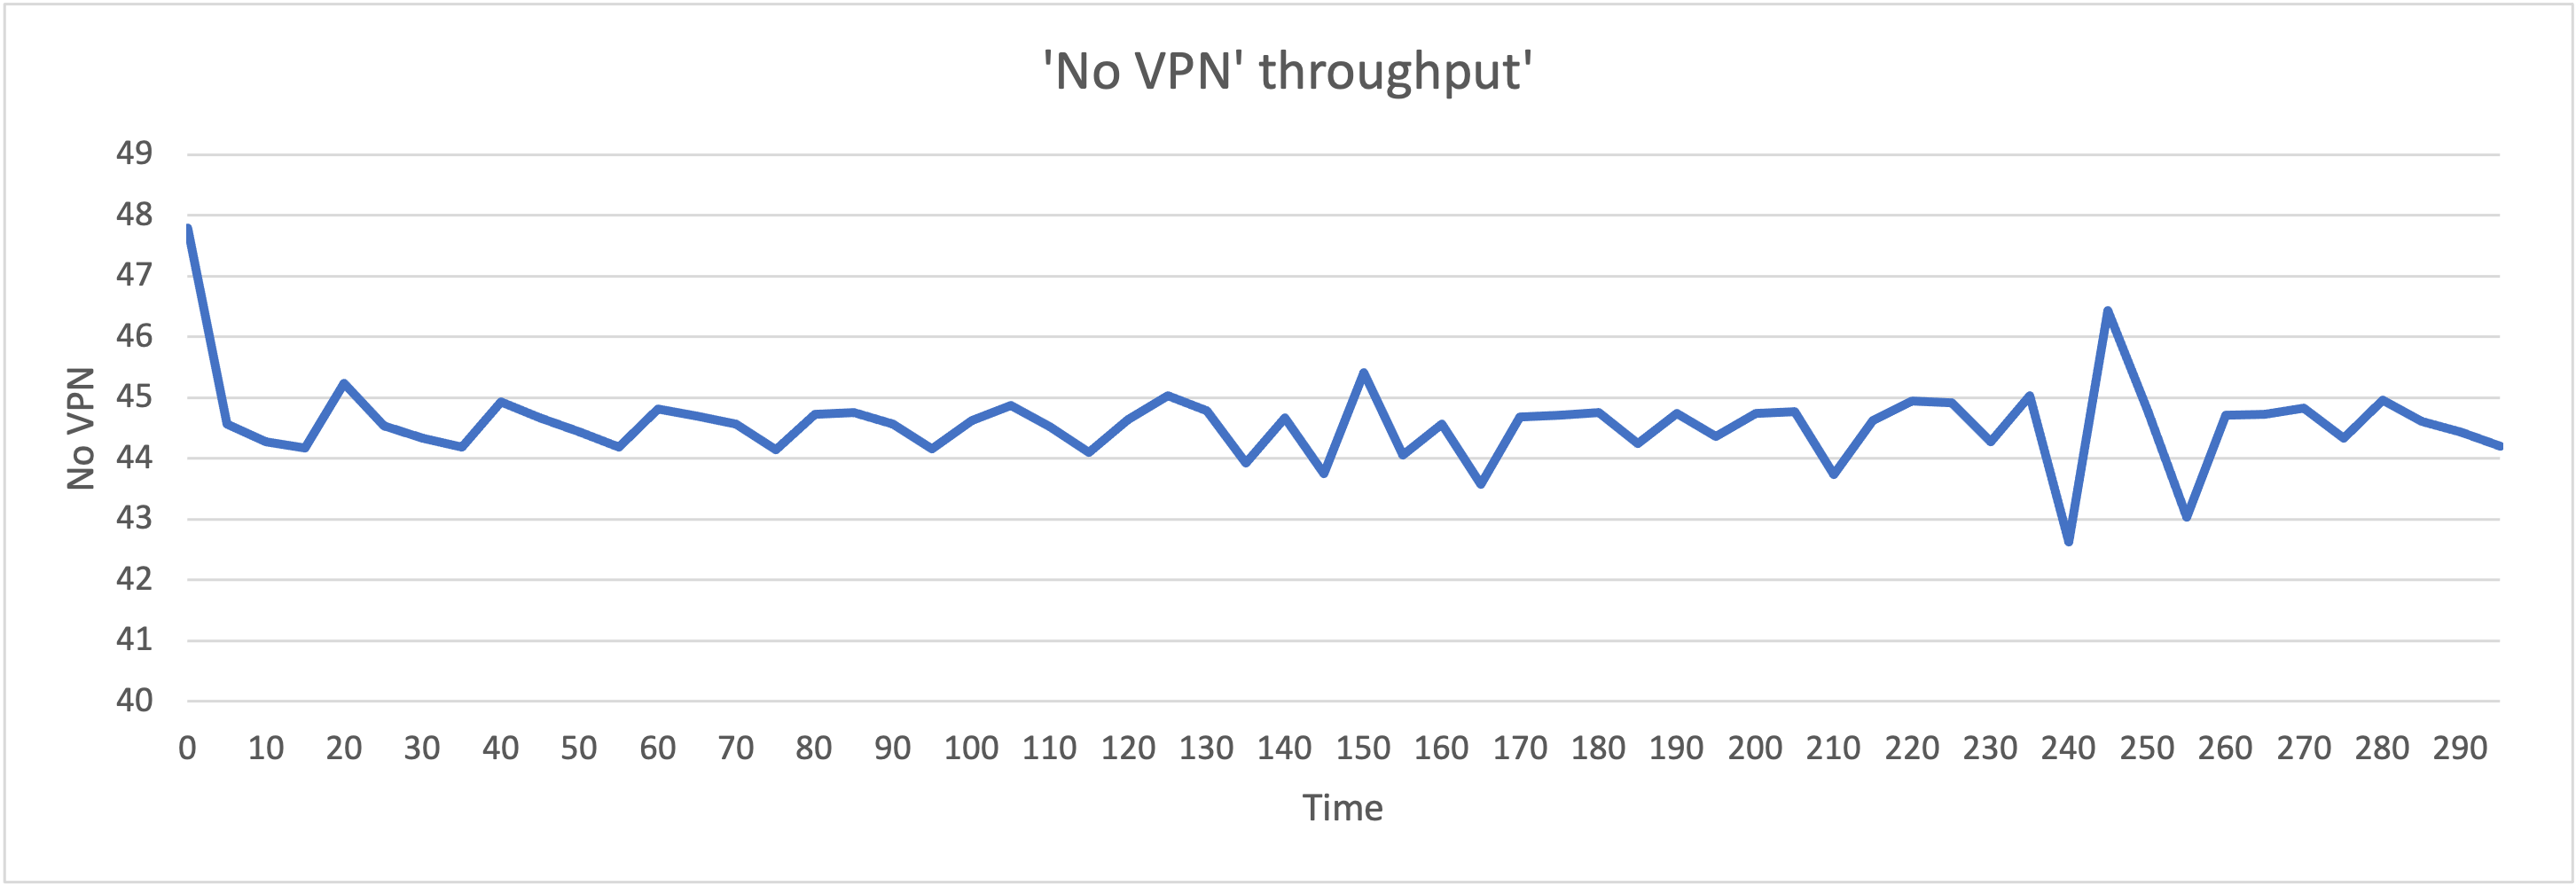
\includegraphics[width=12cm]{figure/vpn_thr.png-1.png}
    \caption{Time in s vs Throughput in Mbit/s}
\end{figure}


\section{Misure con IPSec e IKEv2}
\begin{figure}[ht]
    \centering
    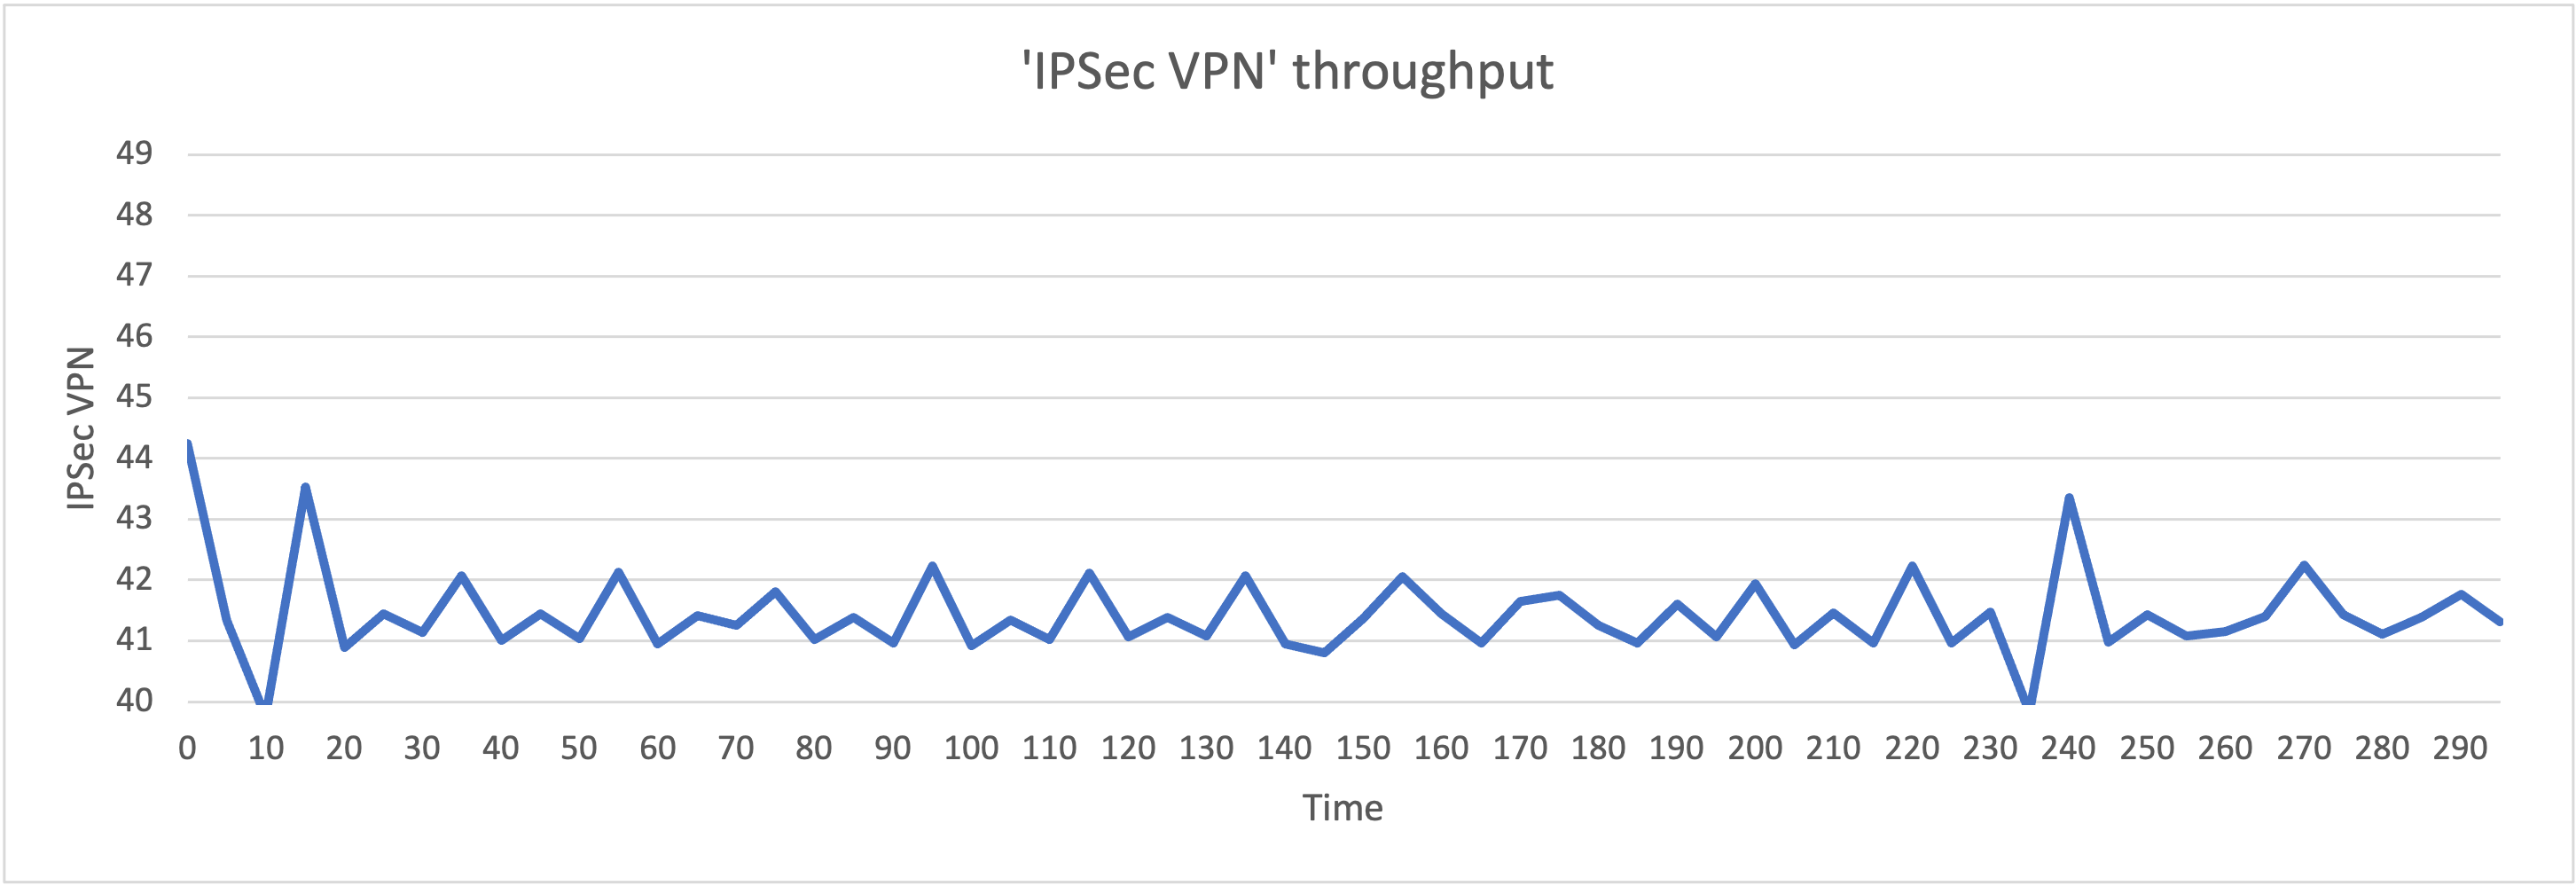
\includegraphics[width=12cm]{figure/vpn_thr.png-2.png}
    \caption{Time in s vs Throughput in Mbit/s}
\end{figure}

\section{Misure con OpenVPN over TCP}
\begin{figure}[ht]
    \centering
    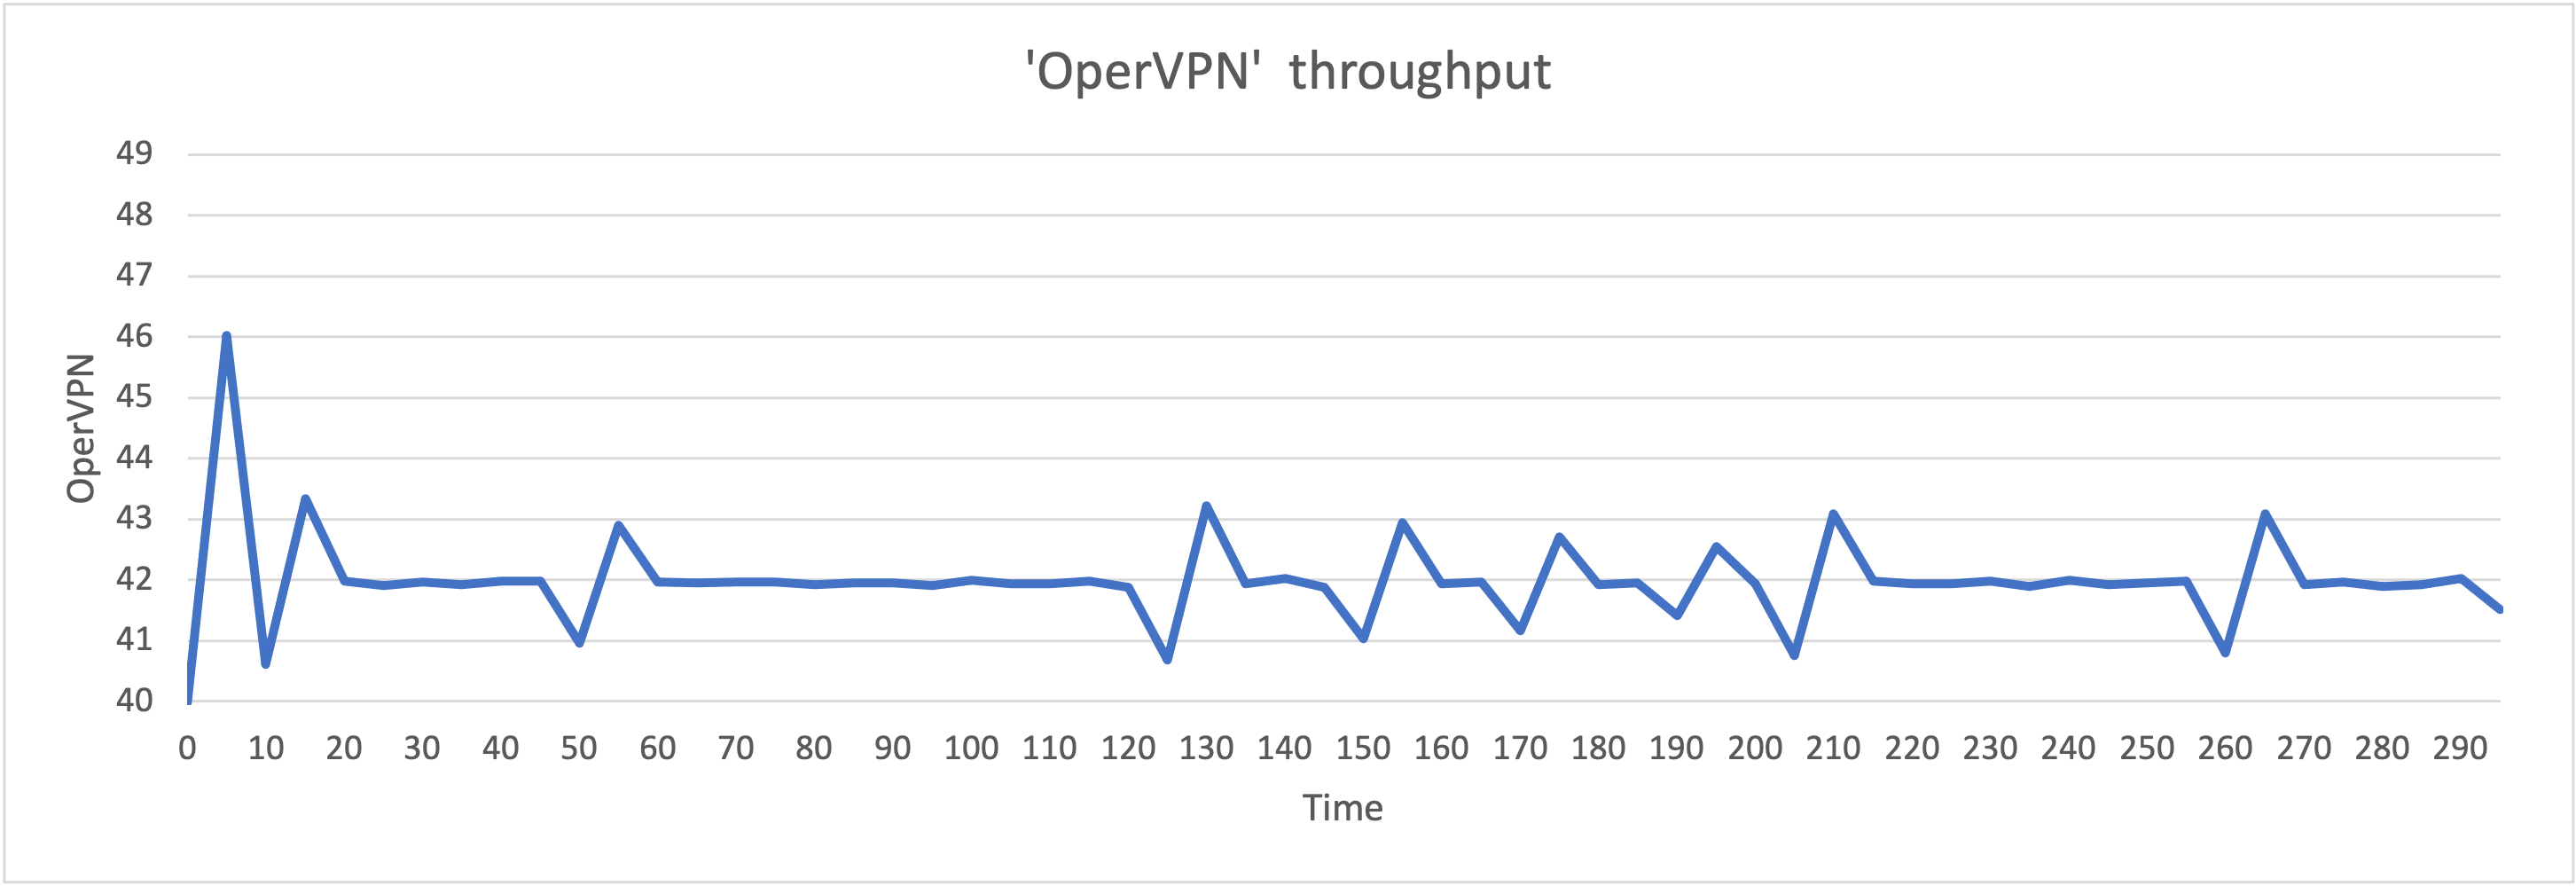
\includegraphics[width=12cm]{figure/vpn_thr.png-3.png}
    \caption{Time in s vs Throughput in Mbit/s}
\end{figure}

\section{Misure con WireGuard}
\begin{figure}[ht]
    \centering
    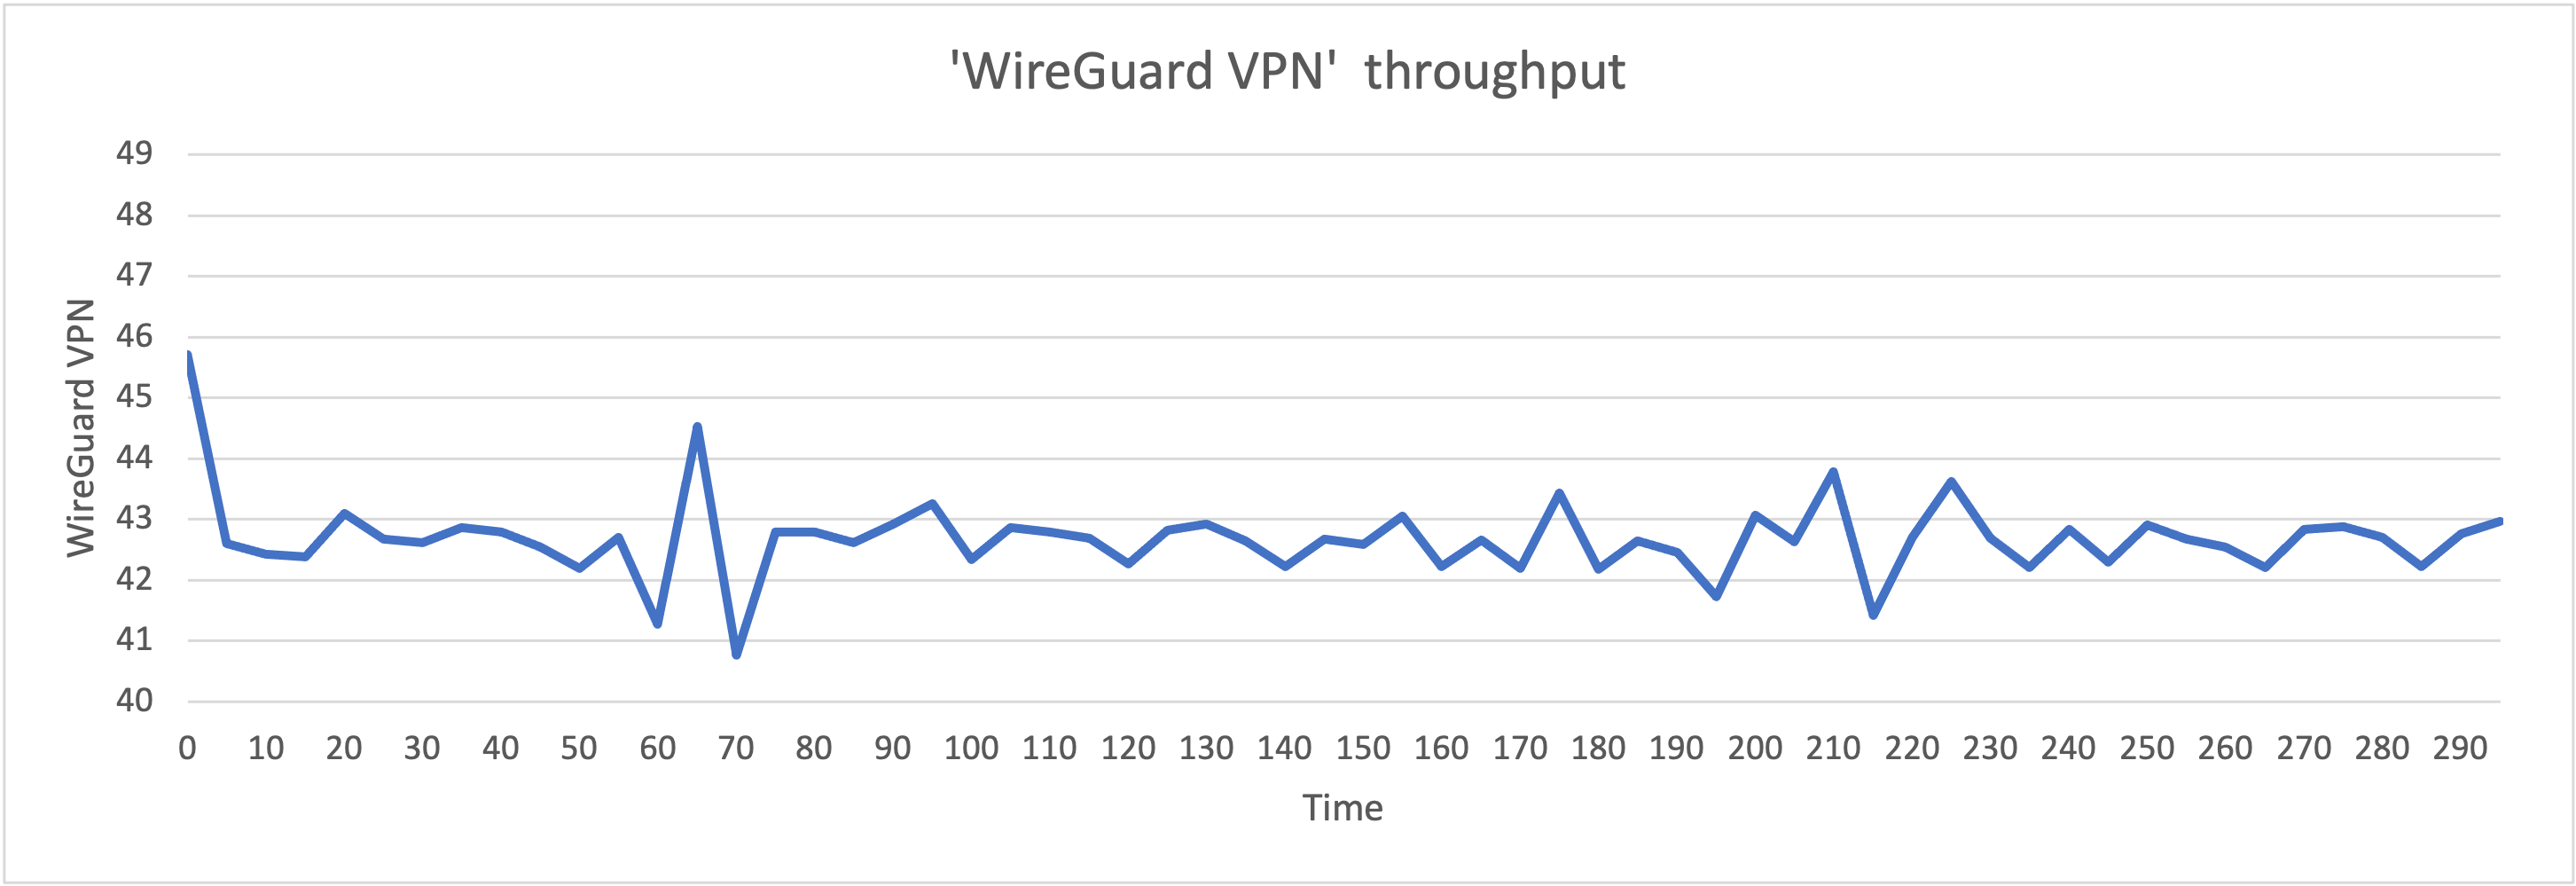
\includegraphics[width=12cm]{figure/vpn_thr.png-4.png}
    \caption{Time in s vs Throughput in Mbit/s}
\end{figure}

\section{Analisi delle misure}
\begin{figure}[ht]
    \centering
    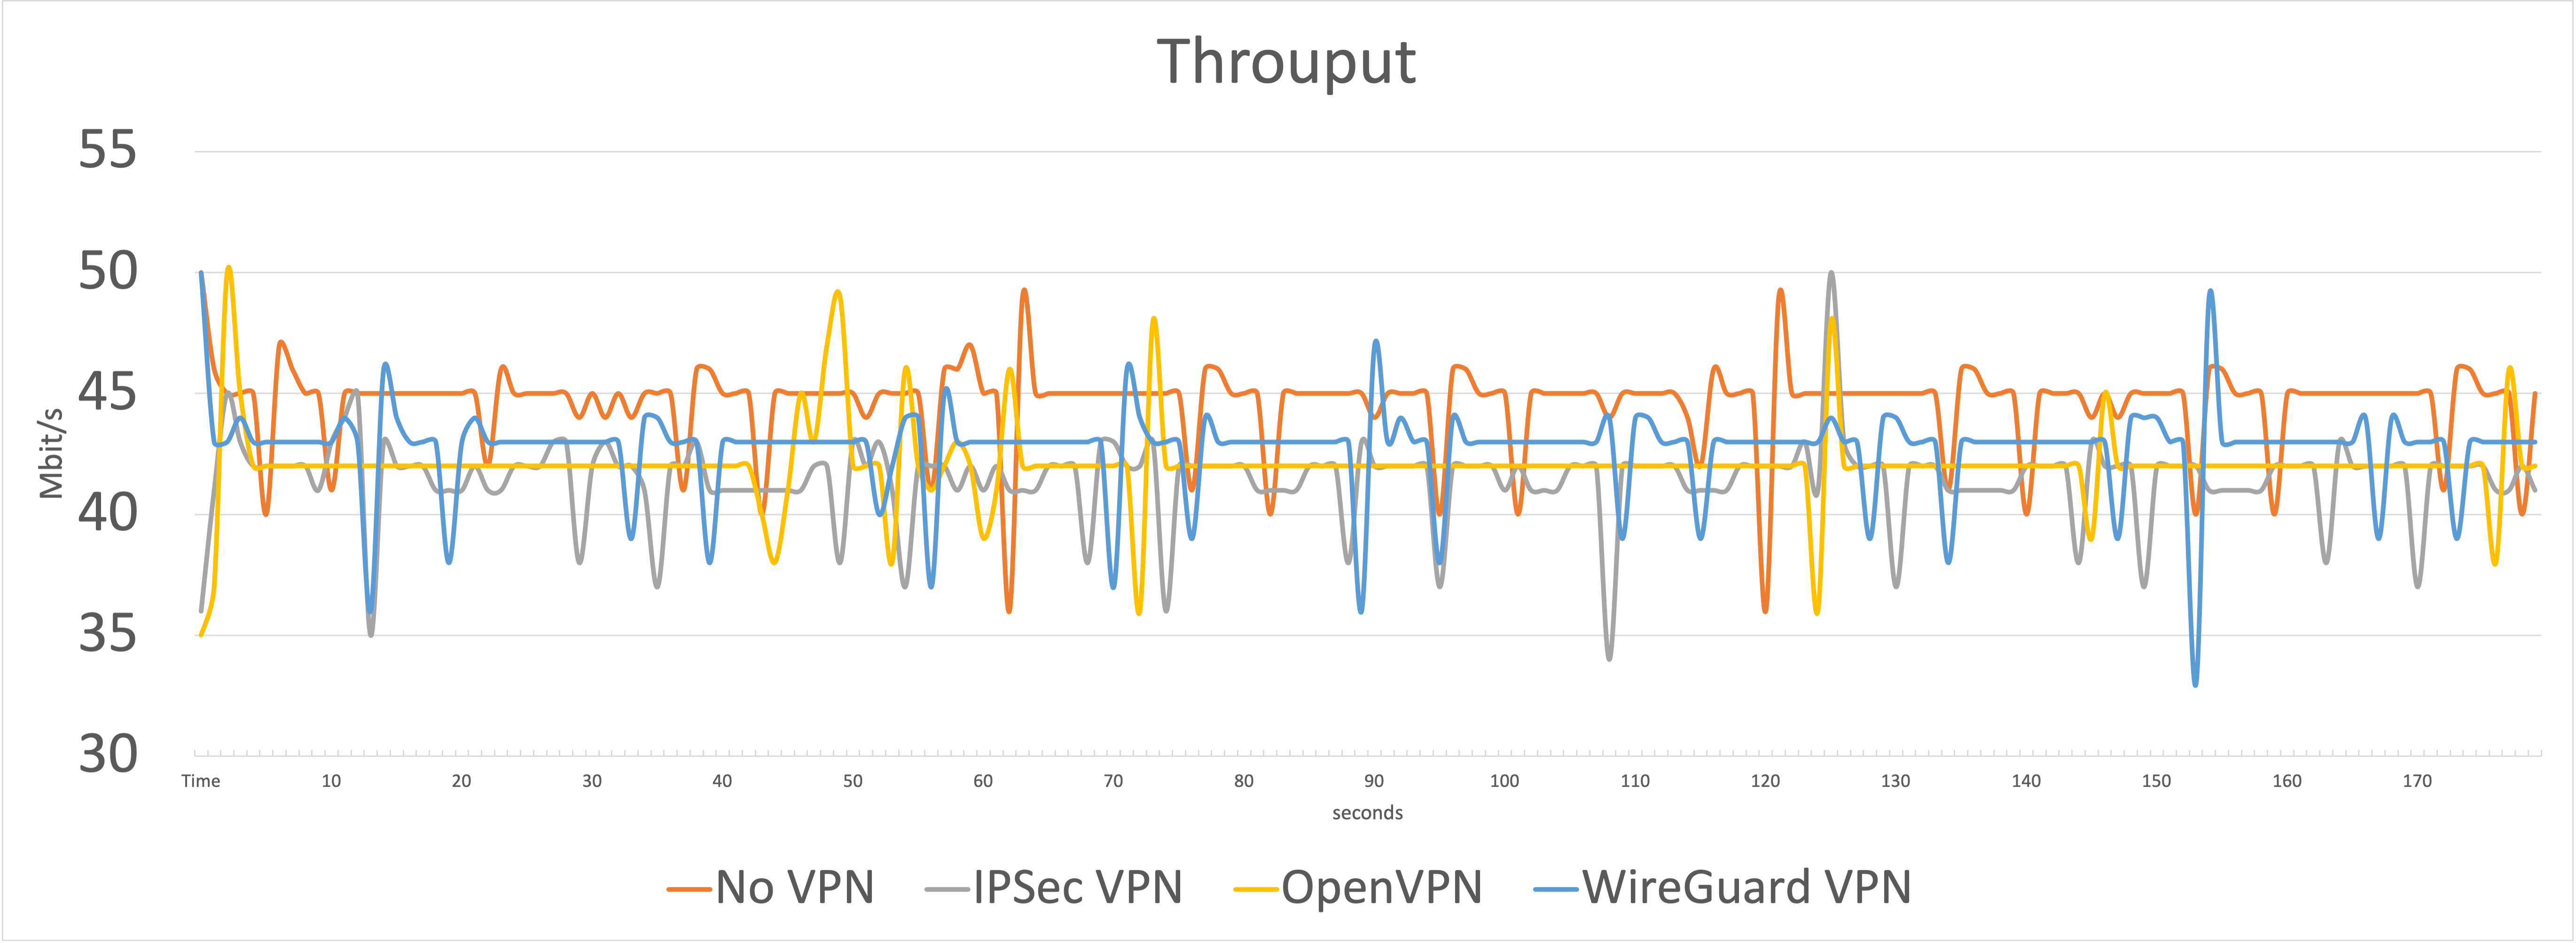
\includegraphics[width=14cm]{figure/rawThroughput.png}
    \caption{Confronto dei throughput grezzi}
\end{figure}

\begin{figure}[ht]
    \centering
    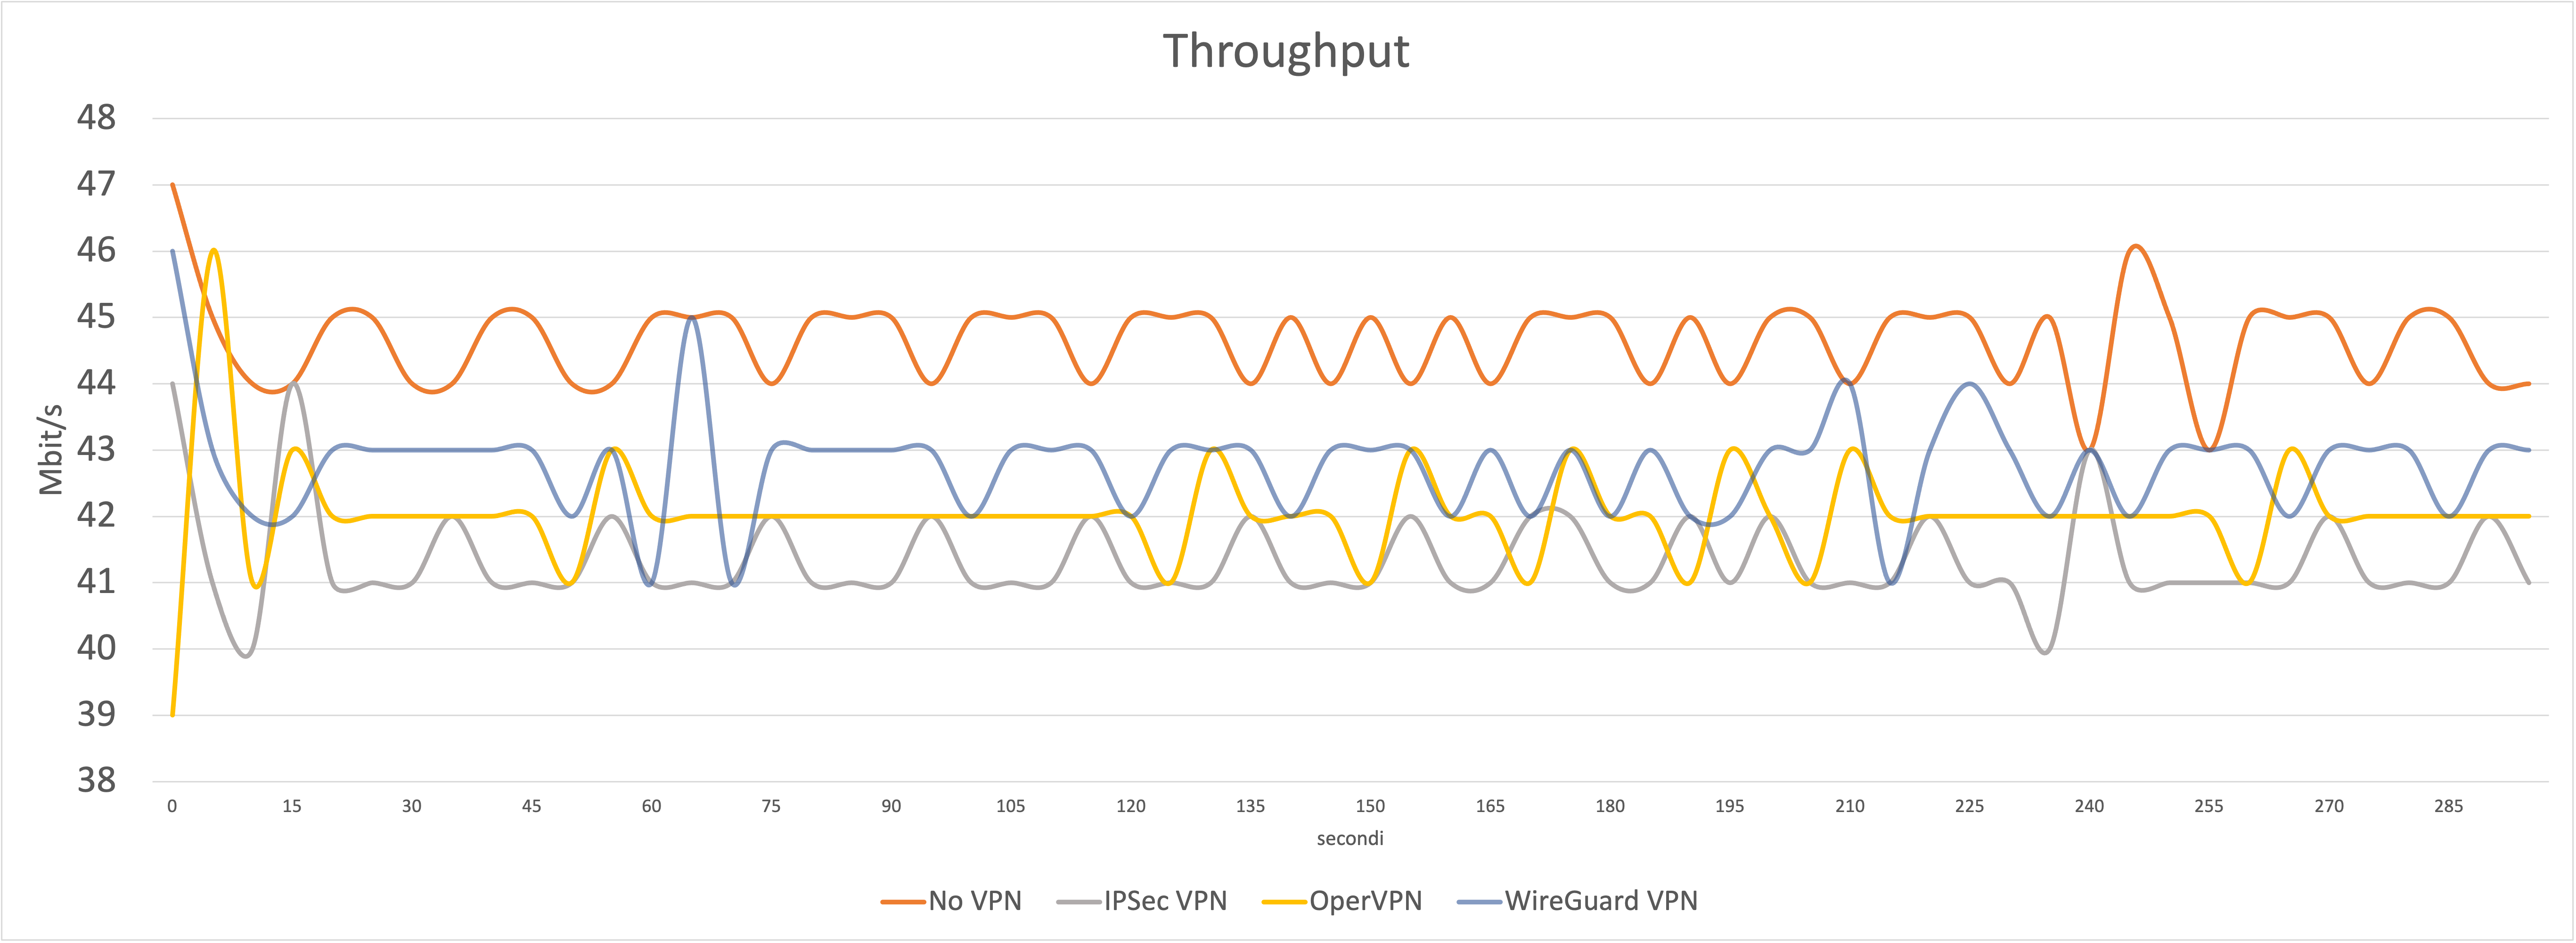
\includegraphics[width=14cm]{figure/fineThroughput.png}
    \caption{Confronto dei throughput raffinati}
\end{figure}

\begin{figure}[ht]
    \centering
    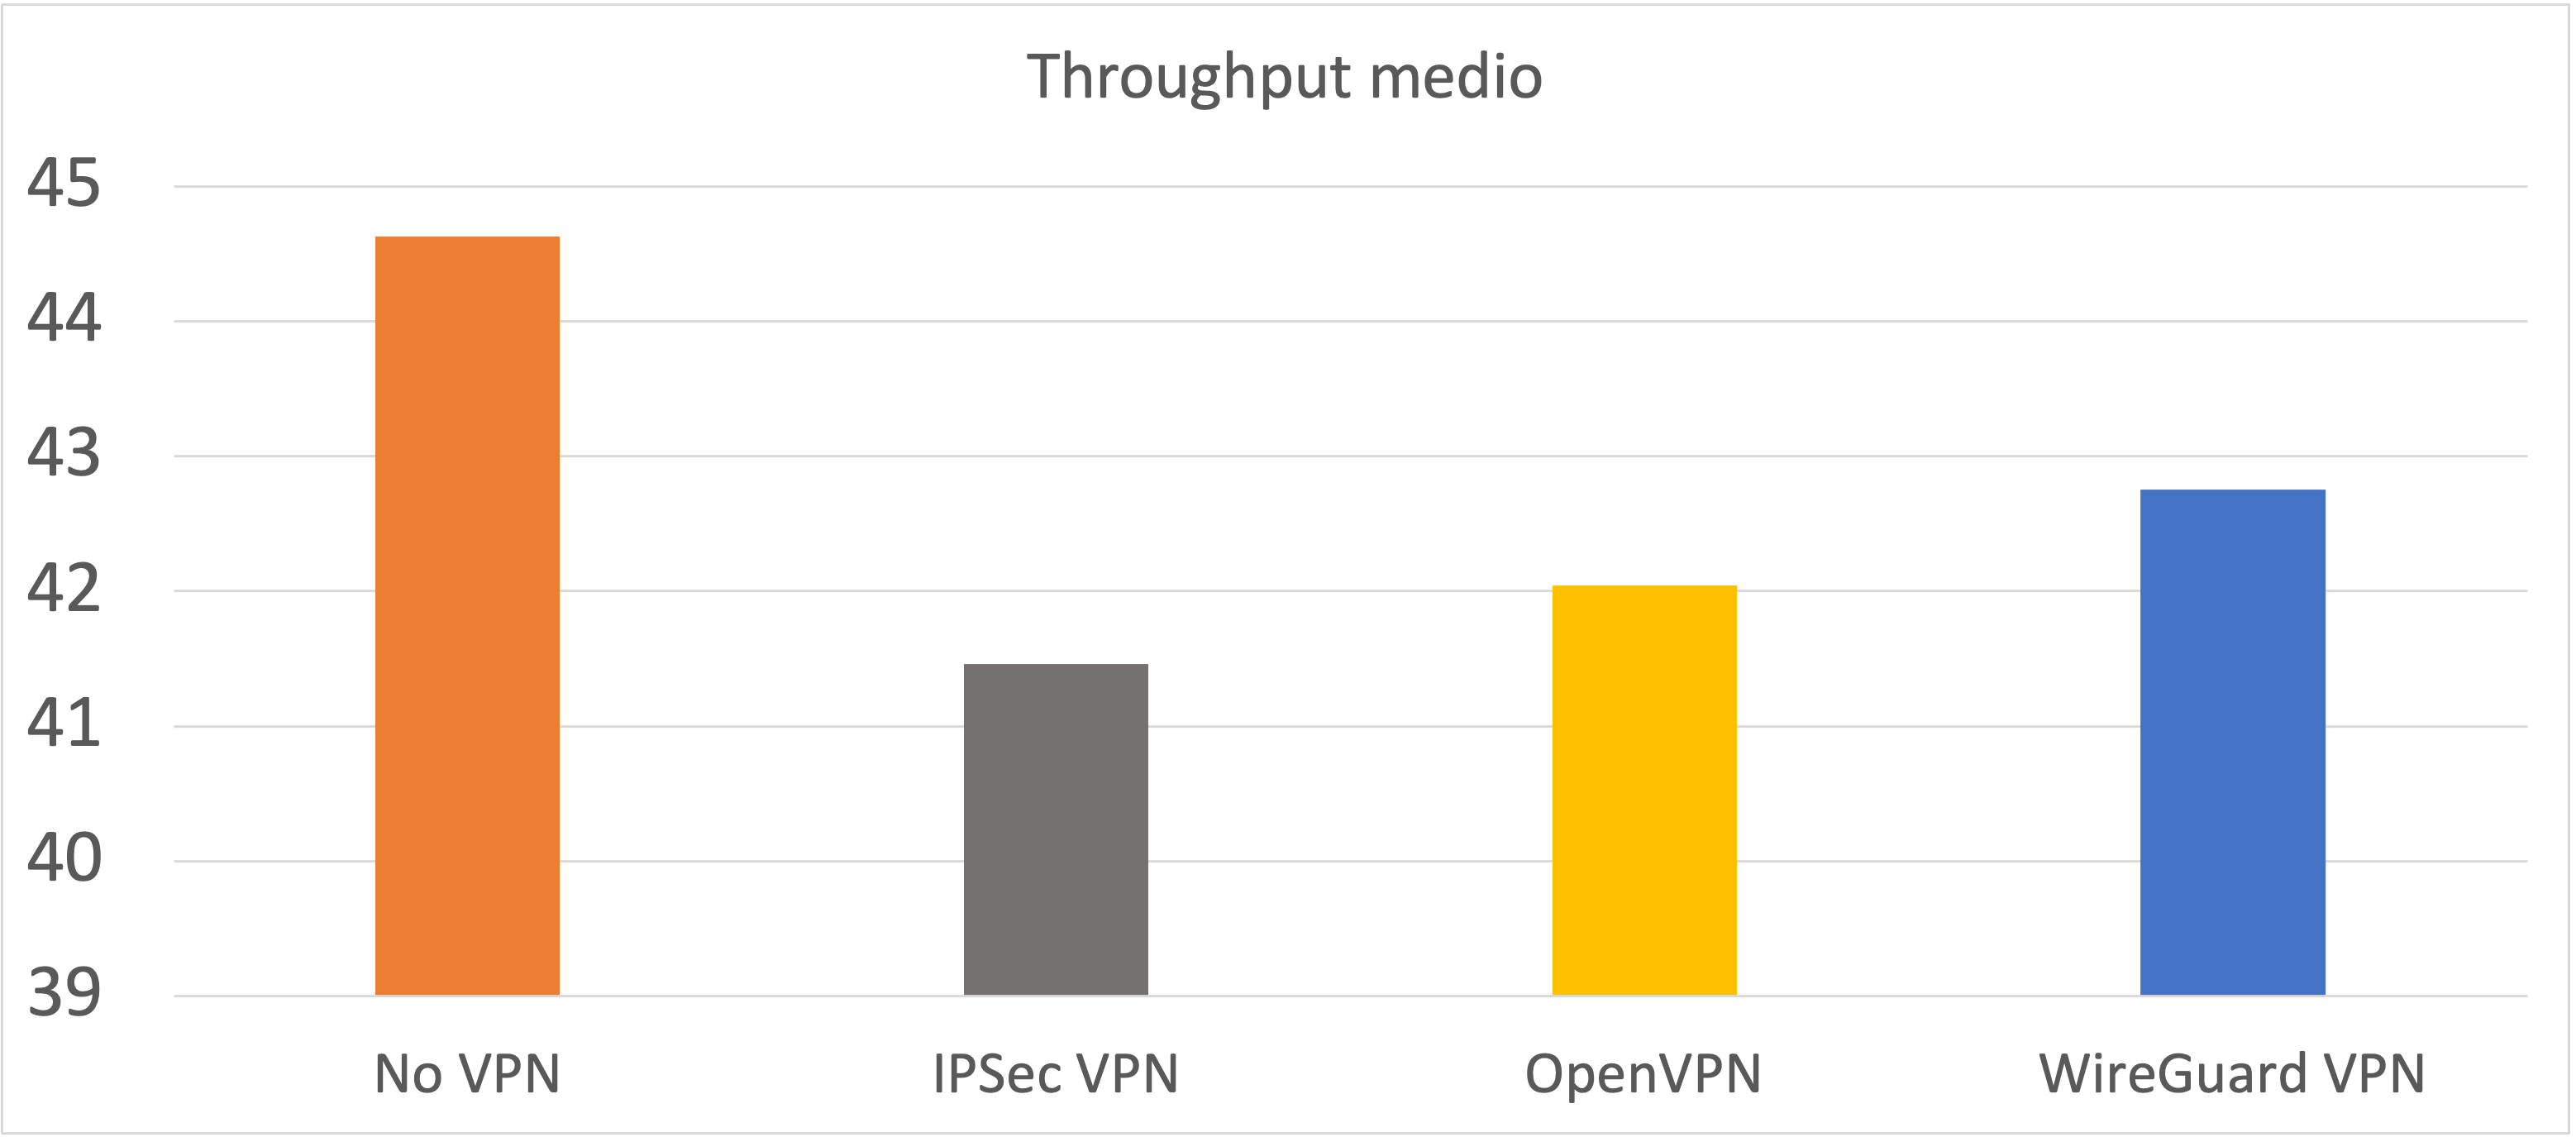
\includegraphics[width=10cm]{figure/avg.png}
    \caption{Confronto dei throughput medi}
\end{figure}